\documentclass[tikz,border=2]{standalone}
\usetikzlibrary{shadows,arrows,shapes,positioning,calc,backgrounds,fit}
% Define the layers to draw the diagram
%
\begin{document}
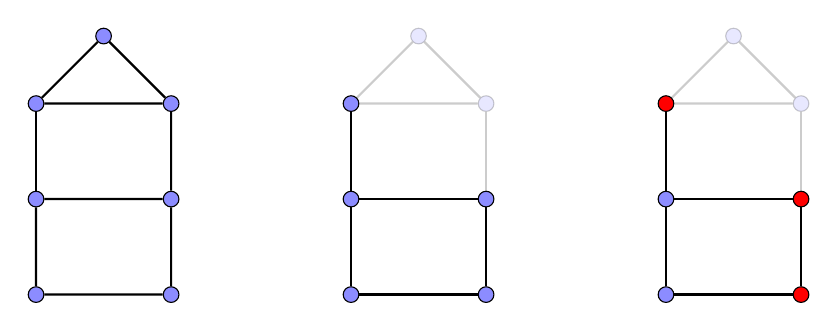
\begin{tikzpicture}
[node distance=1cm,
subdue/.style={opacity=.2},
vertex/.style={shape=circle,draw=black,inner sep=2pt},
infected/.style={vertex,fill=red},
uninfected/.style={vertex,fill=blue!45},
myedge/.style={thick},
dedge/.style={>=latex', shorten >=.0pt, shorten <=.0pt, thick}]
%%
\node (v1) [uninfected] at (0,0) {};
\node (v2) [uninfected,below left=of v1] {};
\node (v3) [uninfected,below right=of v1] {};
\node (v4) [uninfected,below=of v2] {};
\node (v5) [uninfected,below=of v3] {};
\node (v6) [uninfected,below=of v4] {};
\node (v7) [uninfected,below=of v5] {};
\draw[myedge] (v1) -- (v2) -- (v3) -- (v5) -- (v4) -- (v6) -- (v7)
-- (v5);
\draw[myedge] (v1) -- (v3);
\draw[myedge] (v2) -- (v4);
%%
\node (v1) [uninfected,subdue] at (4,0) {};
\node (v2) [uninfected,below left=of v1] {};
\node (v3) [uninfected,subdue,below right=of v1] {};
\node (v4) [uninfected,below=of v2] {};
\node (v5) [uninfected,below=of v3] {};
\node (v6) [uninfected,below=of v4] {};
\node (v7) [uninfected,below=of v5] {};
\draw[myedge,subdue] (v1) -- (v2) -- (v3) -- (v1);
\draw[myedge,subdue] (v3) -- (v5);
\draw[myedge] (v2) -- (v4) -- (v5) -- (v7) -- (v6) -- (v4);
%%
\node (v1) [uninfected,subdue] at (8,0) {};
\node (v2) [infected,below left=of v1] {};
\node (v3) [uninfected,subdue,below right=of v1] {};
\node (v4) [uninfected,below=of v2] {};
\node (v5) [infected,below=of v3] {};
\node (v6) [uninfected,below=of v4] {};
\node (v7) [infected,below=of v5] {};
\draw[myedge,subdue] (v1) -- (v2) -- (v3) -- (v1);
\draw[myedge,subdue] (v3) -- (v5);
\draw[myedge] (v2) -- (v4) -- (v5) -- (v7) -- (v6) -- (v4);
\end{tikzpicture}
{}
\end{document}
